\chapter{Laboratorio 3}
\section{Introduzione}
In questa esperienza di laboratorio, è stato analizzato il circuito di amplificazione \textit{common emitter amplifier} con degenerazione di emettitore, nella versione con alimentazione positiva e negativa e nella versione single-ended (\Fig\ref{fig:commonemitter}).
\begin{figure}[h!]
	\centering
	A
	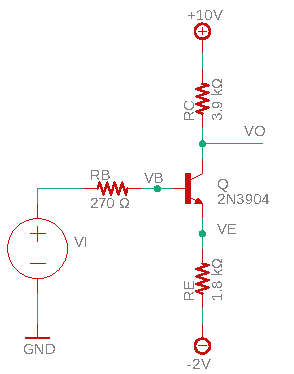
\includegraphics[width=0.4\linewidth]{./OtherFiles/Laboratorio 3/common emitter}
	B
	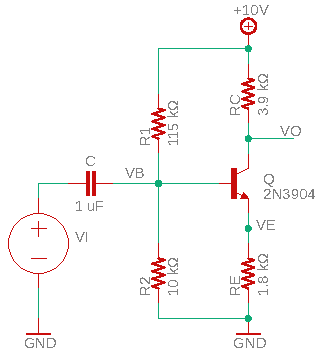
\includegraphics[width=0.4\linewidth]{./OtherFiles/Laboratorio 3/common emitter_se}
	\caption{Schematico del circuito common emitter con degenerazione di emettitore nella versione con alimentazione doppia (A) e singola (B).}
	\label{fig:commonemitter}
\end{figure}

\section{Common emitter amplifier: punto di lavoro}
Prima di procedere alla realizzazione dei circuito analizziamone il punto di lavoro.

Consideriamo prima la versione con alimentazione doppia. Supponiamo il transistor in regione attiva diretta, con corrente di base nulla. Allora la tensione al nodo V\sub{B} sarà nulla (corrente nella resistenza R\sub{B} nulla). Allora, ricordando che $V_{BE}=\SI{-0.7}{\volt}$, si deriva che $V_E=\SI{-0.7}{\volt}$. Per cui, la corrente che attraversa la resistenza R\sub{E} è pari a (legge di Ohm) $I_E=\frac{V_E-(\SI{-2}{\volt})}{R_E}$. Dal bilancio di correnti nel transistor, si ricava che $I_C+I_B=I_E$. Dal momento che la corrente di base è considerata nulla, otteniamo che $I_C=I_E$. Ricaviamo poi V\sub{o} tramite legge di Ohm: $I_C=\frac{\SI{10}{\volt}-V_o}{R_C}$, da cui $V_o= \SI{10}{\volt}-R_C*I_C$. Inoltre, ricordiamo che $g_m=\frac{I_C^*}{\phi_T}$, con $I_C^*$ corrente di collettore stazionaria e $\phi_T\simeq\SI{26}{\milli\volt}$.
\begin{figure}[h!]
	\centering
	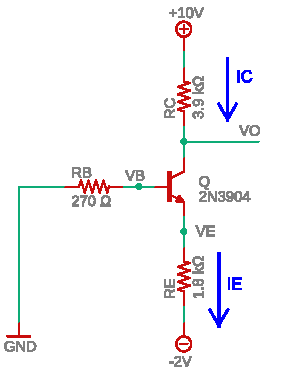
\includegraphics[width=0.4\linewidth]{./OtherFiles/Laboratorio 3/common emitter-punto di lavoro-printout}
	\caption{Analisi del punto di lavoro del circuito common emitter amplifier con alimentazione positiva e negativa.}
	\label{fig:commonemitter_DC}
\end{figure}

Sostituendo i valori utilizzati nel circuito otteniamo i seguenti valori, che saranno da confrontare con quelli misurati sul circuito reale:
\begin{table}[h!]
	\centering
	\begin{tabular}{c|c|c|c|c|c|c}
		\hline
		V\sub{B} [V] & V\sub{E} [V] & V\sub{o} & I\sub{B} [A] & I\sub{E} [mA] & I\sub{C} [mA] & g\sub{m} [A/V]\\ \hline
		0 & -0.7 & 7.183  & 0 & 0.7222 & 0.7222 & 0.0277 \\ \hline
	\end{tabular}
\end{table}
\todo{inserire tabella nel laboratorio 2}

\section{Common emitter amplifier: analisi per piccolo segnale}
\section{Componenti e misure}